% !TEX root = ../main.tex

\section{Related Work}
\label{sec:org2aceb9f}

\todo{look at [[https://www.sciencedirect.com/topics/computer-science/extractive-summarization][extractive summarization]]}

This section will be guided by the previous section's formulation of the multitags problem, we will therefore focus on \emph{algorithm adaptation}, \emph{metrics as losses} and \emph{thresholding}.

\subsection{Algorithm adaptation}
\label{sec:org150a474}

Early representatives of \emph{algorithm adaptation} stem from heterogenous domains of machine learning. Multi-Label k-Nearest Neighbors \cite{ML-KNN}, Multi-Label Decision Tree \cite{ML-DT}, Ranking Support Vector Machine \cite{multilabelSVM} and Backpropagation for Multi-Label Learning \cite{multilabelBackprop}. More recently, two papers introduced the idea of multitask learning for \emph{label prediction} and \emph{label count prediction} for text (ML\(_{\text{NET}}\)) \cite{multitaskLabel} and image \cite{multitaskLabelImages} data. The latter research is loosely catered towards object detection (although not formally presented as such) and is thus out-of-scope: elements in a picture are predicted that tend to be unilabel as defined by the groundtruth (e.g. cat, flower, vase, person, bottle etc.).

\subsection{Metrics as losses}
\label{sec:orgb0a9d21}

Often, machine learning post-training evaluation metrics (e.g. AUROC, F1) are not differentiable. There are motivations \todo{which motivations} for optimizing a model directly on a metric at training time. A general framework for AUC, AUROC and F1 is presented in \cite{optimizableLosses}, but the proposed F1 surrogate remains short of being explicitly derived for stochastic gradient descent. \todo{check again with the authors if I can't get inspired from their work}. Recently, a similar work has been proposed to train a Convolutional Neural Network (CNN) from scratch with a few millions of images and hundreds of labels specifically for multilabel tasks \cite{tencent}. This task is loosely related to object detection, similarly to \cite{multitaskLabelImages} mentioned in the previous paragraph.


% in reformulating loss functions to accomodate sparsity in the data, to optimize directly for the metric at hand or to do thresholding posthoc (see movie posters).

\subsection{Thresholding}
\label{sec:org8295f09}

\emph{thresholding} accross classes or examples can be an issue as soon as the number of labels to predict is unknown. Certain variants of cross-entropy loss accommodate imbalanced label data  \cite{focalLoss}, but remain agnostic towards the number of labels to predict. Solutions have been tailored to that end, starting with determining an ideal global \emph{threshold} depending on use-cases \cite{threshForF1}, or per-class-thresholding after training \cite{moviePosters} and eventually abstracting the threshold away via a \emph{soft-F1} measure \cite{softF1} \todo{say more about this method}. In the latter two cases, the task is to predict genre from movie posters.

\begin{figure}[htbp]
\centering
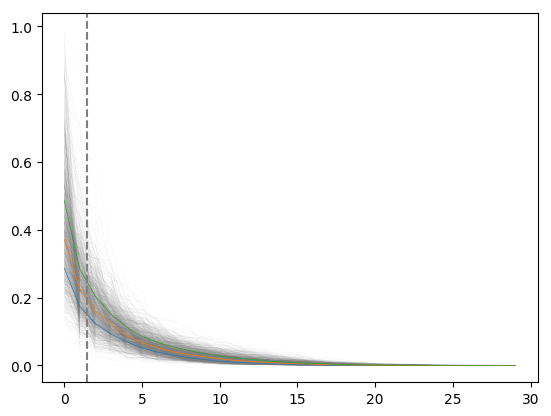
\includegraphics[width=.9\linewidth]{./images/knee.png}
\caption{\label{fig:knee}
\mdr{Why is this figure here, in the related work section?}
Ordered per-label cross-entropy predictions for each example (each grey line) with the median (orange) and IQR (green \& blue) over all examples. Determining a global threshold can be related to visually finding the ``knee'' in that median curve (dotted line).}
\end{figure}

\todo{nicer plot on another dataset (this is from RTL)}

The proposed method is positioned in the lineage of \emph{algorithm adaptation}, using \emph{metric as losses} and allowing for dynamic \emph{thresholding}. 

% We propose a dynamic thresholding mechanism auto-tuned at training time.


% ** weak labels
% (unsure the labels are correct)

% - https://people.cs.pitt.edu/~kovashka/ye_zhang_kovashka_iccv2019_cap2det.pdf


% ** implementations

% *** movies

%  [[https://www.analyticsvidhya.com/blog/2019/04/build-first-multi-label-image-classification-model-python/][movie posters with classes]].

%  They have movie titles in them

% *** pretrained resnet on multilabel

%  https://github.com/Tencent/tencent-ml-images

% What happens when using a Resnet pretrained on multilabels

% *** soft F1 score loss

%  https://github.com/ashrefm/multi-label-soft-f1

% https://www.analyticsvidhya.com/blog/2019/04/build-first-multi-label-image-classification-model-python/



% /Optimizing directly for macro F1: By introducing the macro soft-F1 loss, we could train the model to directly increase the metric we care about: the macro F1-score @ threshold 0.5. We could clearly observe the alignment during training and evaluation on successive epochs. When using this loss, we do not have to tune the decision threshold any more. Imagine a multi-label classification system with hundreds of labels, how unstable the system will be if we have to continuously update the optimal threshold for each label. The macro soft-F1 loss comes to the rescue. By using it, we can keep all thresholds fixed at 0.5 and still get an optimal performance from the training process./


